\chapter{Methodology}\label{chap:methodology}

\begin{quotation}
      ``Observation, reason and experimentation make up what we call the scientific method.''
\end{quotation}
\begin{flushright}
      - Richard P. Feynman
\end{flushright}

So far, this dissertation has provided background information on \acfp{ANN}, \index{heuristic}heuristics, \acp{HH} and probability theory in Chapters \ref{chap:anns} to \ref{chap:probability}. Chapter \ref{chap:bhh} provided the detail of the implementation of the proposed \acs{BHH} with all its components and hyper-parameters. Scientific experimentation can now be conducted. Chapter \ref{chap:introduction} identified a set of empirical goals for this dissertation. The goals of this dissertation include an empirical evaluation of the \acs{BHH}, its behaviour and performance, and a comparison to state of the art low-level \index{heuristic}heuristics. This chapter provides the detailed specification of the methodology that is followed for the empirical process. Details are provided on the implementation of experiments, datasets, selection of hyper-parameters and design decisions. The process by which the results are statistically analysed are also presented. The remainder of the chapter is structured as follows:

\begin{itemize}
      \item \textbf{Section \ref{sec:methodology:overview}} provides a brief overview of the overall empirical process.

      \item \textbf{Section \ref{sec:methodology:datasets}} presents the detail around the datasets that are used.

      \item \textbf{Section \ref{sec:methodology:model}} provides the details of the models (\acs{FFNN}s) that are trained.

      \item \textbf{Section \ref{sec:methodology:heuristics}} presents the detail around the different \index{heuristic}heuristics that are used along with their hyper-parameters.

      \item \textbf{Section \ref{sec:methodology:baseline_bhh}} provides the detail of the configuration of the \acs{BHH} baseline.

      \item \textbf{Section \ref{sec:methodology:performance_measures}} sheds light into the performance evaluation measures that are used.

      \item \textbf{Section \ref{sec:methodology:stopping_conditions}} discusses the stopping conditions that are used.

      \item \textbf{Section \ref{sec:methodology:experiments}} presents the different experimental groups that are executed.

      \item \textbf{Section \ref{sec:methodology:implementation}} sheds light on the implementation and execution of the empirical process.

      \item \textbf{Section \ref{sec:methodology:statistical_analysis}} presents the procedures that are followed for the statistical analysis of the results.

      \item \textbf{Section \ref{sec:methodology:summary}} presents a brief summary of the chapter.
\end{itemize}

\section{Overview of Empirical Process}\label{sec:methodology:overview}

The purpose of the empirical process is to conduct a carefully crafted set of experiments that produce data that can be used to reject of verify a hypothesis about the element under investigation. Chapter \ref{chap:introduction} identified a number of empirical tests to execute. These include:

\begin{itemize}
      \item An empirical study to show that the \Acs{BHH} can effectively be used to train \acp{FFNN}.

      \item An empirical study to investigate the behavioural characteristics of the \Acs{BHH} as it is used to train \acp{FFNN} on an example problem.

      \item An empirical study to critically evaluate the performance of the \Acs{BHH} compared to individual low-level \index{heuristic}heuristics in the \index{heuristic}heuristic space as they are used to train \acp{FFNN} on a number of different problems.
\end{itemize}

These empirical tests represent a set of questions, related to the \acs{BHH}, that need to be answered. The empirical process is designed to answer these questions. The empirical process is structured as follows.

Each empirical test starts with a question to be answered. A hypothesis is formulated for the outcome of the empirical test. The empirical tests are then designed around the implementation of the components under evaluation. Each empirical test defines the configuration of elements and generally include a set of parameters that are altered between experiments. Each experiment is evaluated by means of a performance measurement. In the context of training \acp{FFNN}, the underlying model is trained across a number of datasets. Each dataset is split into a training set comprising of 80\% of the data, and a test set comprising of 20\% of the data. The training set is used to train the model, while the test set is used to evaluate the model's performance on unseen data. Training epochs are split into mini-batch iterations with a specified mini-batch size per dataset. Evaluation takes place at every mini-batch step. Due to the stochastic nature of the experiments, each experiment is repeated over 30 independent runs to provide sufficient sample for statistical certainty about the outcome of the results. Each run contains a different random seed, such that each run is unique. The evaluation data forms the results of the empirical test. These results are analysed for statistical significance, from which findings and conclusions are then made. The null hypothesis is then either rejected or accepted based on these findings.

Details around each of these elements are provided in the following sections.

\section{Datasets}
\label{sec:methodology:datasets}

This section provides the detail around the different datasets that are used throughout the empirical process. These datasets originate from the UCI Machine Learning Repository~\cite{ref:uci:2022}. Datasets are grouped by problem type and include seven classification and seven regression datasets. The classification datasets are given in Table \ref{tab:methodology:datasets:classification} and the regression datasets are given in Table \ref{tab:methodology:datasets:regression} below.

\begin{table}[htb]
      \centering
      \caption{Classification datasets}
      \label{tab:methodology:datasets:classification}%
      \par\bigskip
      \resizebox{\textwidth}{!}{
            \begin{tabular}{ccccccccc}
                  \textbf{dataset} & \textbf{output} & \textbf{types}             & \textbf{attributes} & \textbf{classes} & \textbf{instances} & \textbf{batch} & \textbf{steps} & \textbf{citation}          \\
                  \midrule
                  iris             & multivariate    & real                       & 4                   & 3                & 150                & 16             & 10             & ~\cite{ref:fisher:1936}    \\
                  car              & multivariate    & categorical                & 6                   & 4                & 1728               & 128            & 14             & ~\cite{ref:bohanec:1988}   \\
                  abalone          & multivariate    & categorical, integer, real & 8                   & 28               & 4177               & 256            & 17             & ~\cite{ref:waugh:1995}     \\
                  wine quality     & multivariate    & real                       & 12                  & 11               & 4898               & 256            & 20             & ~\cite{ref:cortez:2009}    \\
                  mushroom         & multivariate    & categorical                & 22                  & 2                & 8214               & 512            & 17             & ~\cite{ref:schlimmer:1987} \\
                  bank             & multivariate    & real                       & 17                  & 2                & 45211              & 512            & 89             & ~\cite{ref:moro:2014}      \\
                  diabetic         & multivariate    & integer                    & 55                  & 3                & 100000             & 1024           & 98             & ~\cite{ref:strack:2014}    \\
            \end{tabular}%
      }
\end{table}%

\begin{table}[htb]
      \centering
      \caption{Regression datasets}
      \label{tab:methodology:datasets:regression}%
      \par\bigskip
      \resizebox{\textwidth}{!}{
            \begin{tabular}{cccccccc}
                  \textbf{dataset}    & \textbf{output}           & \textbf{types} & \textbf{attributes} & \textbf{instances} & \textbf{batch} & \textbf{steps} & \textbf{citation}         \\
                  \midrule
                  fish toxicity       & multivariate              & real           & 7                   & 908                & 64             & 15             & ~\cite{ref:cassotti:2015} \\
                  housing             & univariate                & real           & 13                  & 506                & 32             & 16             & ~\cite{ref:harrison:1978} \\
                  forest fires        & multivariate              & real           & 13                  & 517                & 32             & 17             & ~\cite{ref:cortez:2007}   \\
                  student performance & multivariate              & integer        & 33                  & 649                & 32             & 21             & ~\cite{ref:cortez:2008}   \\
                  parkinsons          & multivariate              & integer, real  & 26                  & 5875               & 256            & 23             & ~\cite{ref:tsanas:2009}   \\
                  air quality         & multivariate, time series & real           & 15                  & 9358               & 256            & 37             & ~\cite{ref:de:2008}       \\
                  bike                & univariate                & integer, real  & 16                  & 17389              & 256            & 68             & ~\cite{ref:fanaee:2014}   \\
            \end{tabular}%
      }
\end{table}%

Details on how the datasets where preprocessed and prepared is given in Appendix \ref{app:datasets}.

\subsection{Class Balancing}

A number of classification datasets given in Table \ref{tab:methodology:datasets:classification} contain an unbalanced representation of classes. The empirical process defined in this dissertation does not apply mechanisms to cater for class balancing, in order to eliminate as many variables and factors in the empirical process as possible. It is therefore suggested that the \acs{BHH} first be studied under the assumption of balanced classes, before applying class balancing techniques. In future research opportunities, class balancing should be utilised.

\section{Models}\label{sec:methodology:model}

All models that are trained in this dissertation follow implementations of shallow \acp{FFNN}, meaning that they only have one hidden layer. The architecture of a model is dependent on the dataset being trained on, the type of optimisation problem, the number of input dimensions and the number of output dimensions. The number of hidden layers used were determined empirically. Weights are initialised by means of \index{Glorot uniform sampling}Glorot uniform sampling~\cite{ref:glorot:2010}. The models and their configuration, as it is used for each dataset, are given in Table \ref{tab:methodology:models:configurations}.

\begin{table}[htb]
      \centering
      \caption{Model configurations}
      \label{tab:methodology:models:configurations}%
      \par\bigskip
      \resizebox{\textwidth}{!}{
            \begin{tabular}{rcccccccc}
                  \textbf{dataset}    & \textbf{inputs} & \textbf{hidden} & \textbf{output} & \textbf{biases} & \textbf{parameters} & \textbf{topology} & \textbf{l1 activation} & \textbf{l2 activation} \\
                  \midrule
                  fish toxicity       & 6               & 3               & 1               & yes             & 25                  & dense             & LReLU ($\alpha = 0.3$) & sigmoid                \\
                  iris                & 4               & 5               & 3               & yes             & 43                  & dense             & LReLU ($\alpha = 0.3$) & softmax                \\
                  air quality         & 12              & 8               & 1               & yes             & 113                 & dense             & LReLU ($\alpha = 0.3$) & sigmoid                \\
                  housing             & 13              & 8               & 1               & yes             & 121                 & dense             & LReLU ($\alpha = 0.3$) & sigmoid                \\
                  wine quality        & 13              & 10              & 7               & yes             & 217                 & dense             & LReLU ($\alpha = 0.3$) & softmax                \\
                  parkinsons          & 21              & 10              & 1               & yes             & 231                 & dense             & LReLU ($\alpha = 0.3$) & sigmoid                \\
                  car                 & 21              & 10              & 4               & yes             & 264                 & dense             & LReLU ($\alpha = 0.3$) & softmax                \\
                  forest fires        & 43              & 16              & 1               & yes             & 721                 & dense             & LReLU ($\alpha = 0.3$) & sigmoid                \\
                  abalone             & 10              & 36              & 28              & yes             & 1432                & dense             & LReLU ($\alpha = 0.3$) & softmax                \\
                  bank                & 51              & 32              & 1               & yes             & 1697                & dense             & LReLU ($\alpha = 0.3$) & softmax                \\
                  bike                & 61              & 32              & 1               & yes             & 2017                & dense             & LReLU ($\alpha = 0.3$) & sigmoid                \\
                  student performance & 99              & 32              & 1               & yes             & 3233                & dense             & LReLU ($\alpha = 0.3$) & sigmoid                \\
                  adult               & 108             & 64              & 1               & yes             & 7041                & dense             & LReLU ($\alpha = 0.3$) & softmax                \\
                  mushroom            & 117             & 64              & 1               & yes             & 7617                & dense             & LReLU ($\alpha = 0.3$) & softmax                \\
                  diabetic            & 2369            & 32              & 3               & yes             & 75939               & dense             & LReLU ($\alpha = 0.3$) & softmax                \\
            \end{tabular}%
      }
\end{table}%

For the classification problems presented in Tables \ref{tab:methodology:datasets:classification} and \ref{tab:methodology:models:configurations}, the softmax activation function is added after training and is not included in the model during training. The loss functions, \acf{SparseCatXE} and \acf{BinXE}, that are used, contain a \index{softmax}softmax function.

\index{heuristic}
\section{Heuristics}\label{sec:methodology:heuristics}

This section provides the details of the low-level \index{heuristic}heuristics that are used in the empirical process. Each of these low-level \index{heuristic}heuristics are implemented as standalone \index{heuristic}heuristics and are also included in the \index{heuristic pool}heuristic pool of the \acs{BHH}. Table \ref{tab:methodology:heuristics} contains a list of all the standalone, low-level \index{heuristic}heuristics that are used as well as their hyper-parameter configurations.

% Table generated by Excel2LaTeX from sheet 'BHH Baseline'
\begin{table}[htbp]
      \centering
      \caption{Low-level \index{heuristic}heuristics and their hyper-parameter configurations.}
      \label{tab:methodology:heuristics}%
      \par\bigskip
      \resizebox{0.7\textwidth}{!}{

            \begin{tabular}{llll}
                  \textbf{heuristic} & \textbf{configuration}    & \textbf{value} & \textbf{citation}          \\
                  \midrule
                  sgd                & learning rate             & 0.1 (0.01)     & ~\cite{ref:sutskever:2013} \\
                  momentum           & learning rate             & 0.1 (0.01)     & ~\cite{ref:sutskever:2013} \\
                                     & momentum                  & 0.9            &                            \\
                  nag                & learning rate             & 0.1 (0.01)     & ~\cite{ref:sutskever:2013} \\
                                     & momentum                  & 0.9            &                            \\
                  adagrad            & learning rate             & 0.1 (0.01)     & ~\cite{ref:duchi:2011}     \\
                                     & epsilon                   & 1E-07          &                            \\
                  rmsprop            & learning rate             & 0.1 (0.01)     & ~\cite{ref:hinton:2012}    \\
                                     & rho                       & 0.95           &                            \\
                                     & epsilon                   & 1E-07          &                            \\
                  adadelta           & learning rate             & 1.0 (0.95)     & ~\cite{ref:zeiler:2012}    \\
                                     & rho                       & 0.95           &                            \\
                                     & epsilon                   & 1E-07          &                            \\
                  adam               & learning rate             & 0.1 (0.01)     & ~\cite{ref:kingma:2014}    \\
                                     & beta1                     & 0.9            &                            \\
                                     & beta2                     & 0.999          &                            \\
                                     & epsilon                   & 1E-07          &                            \\
                  pso                & population size           & 10             & ~\cite{ref:van:2010}       \\
                                     & learning rate             & 1.0 (0.9)      &                            \\
                                     & inertia weight (w)        & 0.729844       &                            \\
                                     & cognitive control (c1)    & 1.49618        &                            \\
                                     & social control (c2)       & 1.49618        &                            \\
                                     & velocity clip min         & -1.0           &                            \\
                                     & velocity clip max         & 1.0            &                            \\
                  de                 & population size           & 10             & ~\cite{ref:mezura:2006}    \\
                                     & selection strategy        & best           &                            \\
                                     & xo strategy               & exp            &                            \\
                                     & recombination probability & 0.9 (0.1)      &                            \\
                                     & beta                      & 2.0 (0.1)      &                            \\
                  ga                 & population size           & 10             & ~\cite{ref:lambora:2019}   \\
                                     & selection strategy        & rand           &                            \\
                                     & xo strategy               & bin            &                            \\
                                     & mutation rate             & 0.2 (0.05)     &                            \\
            \end{tabular}%
      }
\end{table}%

Note from Table \ref{tab:methodology:heuristics} that values that are configured to make use of a decay schedule are presented with the initial value first and the decay rate in brackets next to it. The number of steps is the total number of mini-batch training steps that are executed for that particular dataset.

Furthermore, it should be noted that a learning rate was added to \acs{PSO} as an attempt to avoid overshooting solutions later in the training process. A learning rate parameter does not traditionally form part of \acs{PSO}, but was found to be useful. The position update step for \acs{PSO} using a learning rate is then defined as

\begin{equation}
      \label{eq:heuristics:pso:position_learning_rate}
      \begin{split}
            x_{ij}(t+1) = x_{ij}(t) + \eta v_{ij}(t+1)
      \end{split}
\end{equation}

where $\eta$ is the added learning rate with $0 \leq \eta \leq 1, \eta \in \mathbb{R}$.

Section \ref{sec:bhh:heuristic:proxies} presented the concept of a mapping of proxied \index{heuristic}heuristic state update operations. The mapping of proxied \index{heuristic}heuristic state update operations implemented by the \acs{BHH} in the empirical process is given in Figure \ref{fig:methodology:heuristics:proxies}.


\begin{figure}[htbp]
      \centering
      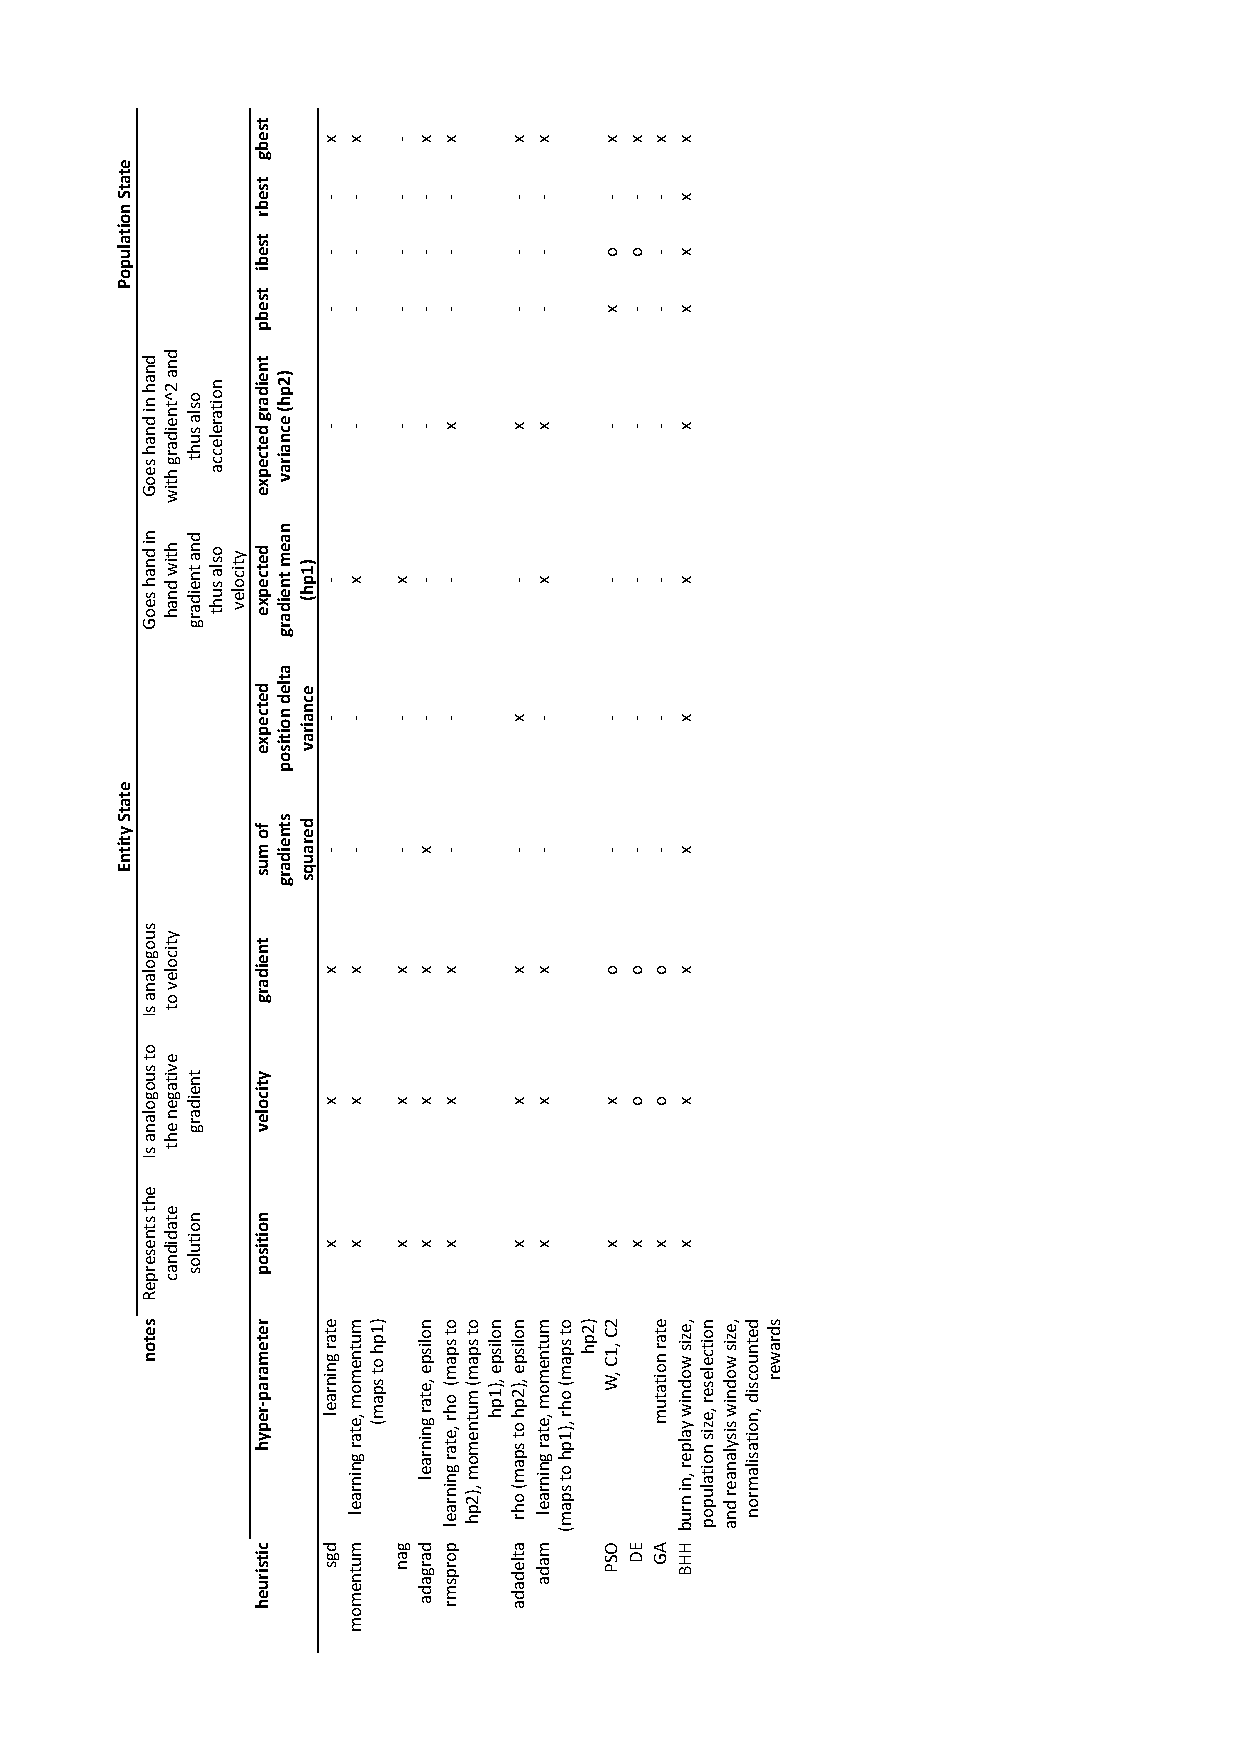
\includegraphics[width=0.7\textwidth]{images/bhh_heuristic_proxies.pdf}
      \caption{Mapping of proxied heuristic state update operations as implemented by the \acs{BHH}}
      \label{fig:methodology:heuristics:proxies}%
\end{figure}


In Figure \ref{fig:methodology:heuristics:proxies}, cells containing \textbf{x} indicate that the associated \index{heuristic}heuristic implements that particular state parameter explicitly, and cells containing \textbf{o} indicate that the state parameter is implicitly implemented as part of the \acs{BHH} algorithm. The required mapping of proxied \index{heuristic}heuristic state operations is then implemented as a lookup of the table presented in Figure \ref{fig:methodology:heuristics:proxies}.

\section{BHH Baseline}\label{sec:methodology:baseline_bhh}

The \acs{BHH} baseline is a name given to a specific configuration of the \acs{BHH} which, during development, has been found to provide a reasonable baseline performance. The baseline configuration is used as the cornerstone configuration from which all other \index{heuristic}heuristics and their configurations are evaluated. The \acs{BHH} baseline is also used for the behavioural study of the \acs{BHH}. The \acs{BHH} baseline configuration is given in Table \ref{tab:methodology:bhh_baseline_configuration}.

% Table generated by Excel2LaTeX from sheet 'BHH Baseline'
\begin{table}[htb]
      \centering
      \caption{The \acs{BHH} baseline configuration as it is used in the empirical study.}
      \label{tab:methodology:bhh_baseline_configuration}%
      \par\bigskip
      \resizebox{0.65\textwidth}{!}{
            \begin{tabular}{rrcc}
                  \multicolumn{1}{c}{\textbf{hyper-heuristic}} & \multicolumn{1}{c}{\textbf{variant}} & \textbf{configuration} & \textbf{value} \\
                  \midrule
                  \multicolumn{1}{l}{bhh}                      & \multicolumn{1}{l}{baseline}         & heuristic pool         & all            \\
                                                               &                                      & population             & 5              \\
                                                               &                                      & credit                 & ibest          \\
                                                               &                                      & burn in                & 0              \\
                                                               &                                      & reselection            & 10             \\
                                                               &                                      & replay                 & 10             \\
                                                               &                                      & reanalysis             & 10             \\
                                                               &                                      & normalise              & false          \\
                                                               &                                      & discounted rewards     & false          \\
            \end{tabular}%
      }
\end{table}%

In Table \ref{tab:methodology:bhh_baseline_configuration}, the \index{heuristic}heuristic pool configuration that is used, is referred to as \textit{all}. The \textit{all} configuration refers to a configuration where the \index{heuristic pool}heuristic pool contains all the low-level \index{heuristic}heuristics as presented in Section \ref{sec:methodology:heuristics}, including all gradient-based \index{heuristic}heuristics and \index{meta-heuristic}meta-heuristics.


\section{Performance Measures}\label{sec:methodology:performance_measures}

This section provides the performance measures that are used to evaluate the different experimental runs during the empirical process. Chapter \ref{chap:anns} provided a number of loss functions. These loss functions are used to measure the performance of the \acp{FFNN} being trained. In this dissertation, \acs{BinXE} is used for classification problems with two classes and \acs{SparseCatXE} is used for classification problems with more than two classes. For the classification problems, accuracy is also measured. Accuracy refers to the proportion of correct classifications. For regression problems, the \acs{RMSE} is used as a performance metric.

The test set is used as a validation set during training. All performance metrics are measured for the training set as well as the test/validation set during training. As such, a divergence in performance metrics between the training and test/validation set is used to evaluate for overfitting during the training process.

After training has been completed, the \textit{average rank}, based on test loss, for all configurations, is calculated at each mini-batch step. A total of 30 independent runs with different random seed configurations are executed for each empirical test. The test loss metric and average rank are then statistically analysed across all runs, and are used to derive findings and conclusions.

\section{Stopping Conditions}\label{sec:methodology:stopping_conditions}

This section provides the stopping conditions that are used during the empirical process. For this dissertation, the \textit{maximum epoch} stopping condition is used, where a fixed, maximum number of training steps and epochs are executed and training is not halted until the maximum number of epochs have been reached. \acp{FFNN} are trained for a maximum of 30 epochs. Early stopping is a technique where training is stopped when the \index{heuristic}heuristic is not able to improve the performance of the \acs{FFNN} for a number of steps. If the performance has not improved, the training is halted and the last known best model weights are restored. Early stopping is not implemented for the empirical process in this dissertation. This design decision is made so that the behaviour of the \acs{BHH} can be studied beyond the point of optimal results.


\section{Experiments}
\label{sec:methodology:experiments}

This section presents the experimental groups that are executed in the empirical process. Three main experimental groups are formulated. Each of these are discussed in more detail in the following sections.


\subsection{Behavioural Case Study}
\label{sec:methodology:experiments:case_study}

The behavioural case study analyses the behaviour of the \acs{BHH} baseline configuration as it relates to an example problem dataset, across 30 independent runs. The example problem dataset is the iris dataset, presented in Table \ref{tab:methodology:datasets:classification}. The behavioural case study is meant to provide an introductory analysis of the inner workings of the \acs{BHH} and includes analysis of the selection mechanism, as well as the perturbative nature of the \acs{BHH}. The behavioural case study is used to determine if the \acs{BHH} is learning and that selection is indeed biasing towards better performance. These observations also provide an opportunity to observe the outcome of the perturbative nature of the \acs{BHH}, which includes proxied \index{heuristic}heuristic update step operations.

The behavioural case study provides an implementation of the \acs{BHH} baseline which, by default, has a replay window size of 10. The baseline configuration is provided and compared to an implementation of a \acs{BHH} configuration where the replay window size is large (250), as well as an implementation of the \acs{BHH} using the \textit{symmetric} credit assignment strategy. The large replay window size configuration is used to show the behaviour of the \acs{BHH} when it has access to a large number of performance log samples, which increases the statistical certainty of the learning outcome. The \acs{BHH} configuration that uses the \textit{symmetric} credit assignment strategy is used to illustrate the behaviour of the \acs{BHH} where no performance bias takes place and thus, no learning occurs.

\subsection{Standalone Heuristics}
\label{sec:methodology:experiments:standalone_optimisers}

For the standalone \index{heuristic}heuristics experimental group, the \index{heuristic}heuristics, as presented in Section \ref{sec:methodology:heuristics}, are used along with their specified hyper-parameters. Each of these standalone low-level \index{heuristic}heuristics are compared to that of the \acs{BHH} baseline configuration, across all datasets.

The intent of the standalone \index{heuristic}heuristics experimental group is to determine if the \acs{BHH} baseline configuration can generalise to multiple problems in comparison to individual low-level \index{heuristic}heuristics.

Additional to the \acs{BHH} baseline configuration, two more \acs{BHH} configurations are included. These include \acs{BHH} configurations where the \index{heuristic pool}heuristic pool only makes use of gradient-based \index{heuristic}heuristics, and a configuration where the \index{heuristic pool}heuristic pool only makes use of \acp{MH}. The intent behind the inclusion of these configurations is to determine the effectiveness of multi-method approaches in the \index{heuristic pool}heuristic pool as it applies to training \acp{FFNN}.

\subsection{BHH Variants}
\label{sec:methodology:experiments:bhh_variants}

This section provides the details of the experimental group that focuses on \acs{BHH} variants and the effect that different hyper-parameter configurations can have on the outcome of the \acs{BHH}. The different variants of the \acs{BHH} and their possible configurations are given in Table \ref{tab:methodology:experiments:bhh_variants}.

\begin{table}[htb]
      \centering
      \caption{BHH variants and their configuration}
      \label{tab:methodology:experiments:bhh_variants}%
      \par\bigskip
      \resizebox{0.9\textwidth}{!}{
            \begin{tabular}{rcc}
                  \multicolumn{1}{c}{\textbf{hyper-heuristic}} & \textbf{variant}   & \textbf{values}                       \\
                  \midrule
                  \multicolumn{1}{l}{bhh}                      & heuristic pool     & all, gd, mh                           \\
                                                               & population         & 5, 10, 15, 20, 25                     \\
                                                               & credit             & ibest, pbest, rbest, gbest, symmetric \\
                                                               & reselection        & 1, 5, 10, 15, 20                      \\
                                                               & replay             & 1, 5, 10, 15, 20                      \\
                                                               & reanalysis         & 1, 5, 10, 15, 20                      \\
                                                               & burn in            & 0, 5, 10, 15, 20                      \\
                                                               & normalise          & false, true                           \\
                                                               & discounted rewards & false, true                           \\
            \end{tabular}%
      }
\end{table}%

In Table \ref{tab:methodology:experiments:bhh_variants}, the \index{heuristic pool}heuristic pool configuration \textit{gd} refers to the \index{heuristic pool}heuristic pool configuration where only gradient-based \index{heuristic}heuristics are included, and \textit{mh} refers to the \index{heuristic pool}heuristic pool configuration where only \acp{MH} are included.

\section{Statistical Analysis}
\label{sec:methodology:statistical_analysis}

This section provides the detail of the process that is used to execute the statistical analysis of the results.

Various experimental groups and configurations have been presented in Sections \ref{sec:methodology:experiments:case_study}, \ref{sec:methodology:experiments:standalone_optimisers} and \ref{sec:methodology:experiments:bhh_variants}. The results from each of these experimental groups are statistically analysed. To ensure that there are sufficient samples for statistical analysis, each experiment and configuration is trained for 30 epochs and is repeated over 30 runs, for each of the fourteen datasets. The experimental results contain performance evaluation data for the training and testing datasets, and includes loss and accuracy measurements. Statistical analysis is executed on the results from the testing datasets. An average rank is calculated across all 30 runs, for all experimental groups and configurations, at each step, for every epoch of training. Each run is executed using a unique random seed, such that each run is identical in its setup and configuration, but unique between runs.

The evaluation of outcome is based on the aggregated statistical results as mentioned above. A descriptive analysis is executed on the spread of the data. The results are analysed and checked for overfitting and outliers are identified. The skewness of the results is evaluated per dataset and the \index{Shapiro-Wilk}Shapiro-Wilk test for normality~\cite{ref:shapiro:1965} ($\alpha$ = 0.001) is used to determine if the results are normally distributed. Furthermore, the \index{Levene}Levene's test for equality of variance~\cite{ref:levene:1961} ($\alpha$ = 0.001) is used. The output of the full statistical analysis is presented in Appendix \ref{app:statistical_analysis}.

Dependent on the outcomes of the above statistical tests, the appropriate statistical significance test is then executed. For experiments where there are only two configurations, the Mann-Whitney U\index{Mann-Whitney U} independent samples t-Test~\cite{ref:mann:1947} ($\alpha$ = 0.001) is executed. For experiments with three or more configurations, the \acs{ANOVA} statistical test~\cite{ref:fisher:1921} ($\alpha$ = 0.001) is used. The\index{Kruskal-Wallis} Kruskal-Wallis ranked non-parametric test~\cite{ref:kruskal:1952} for statistical significance ($\alpha$ = 0.001) is used for cases where data is not normally distributed.

Regardless of the statistical test that is used, a post-hoc Tukey honest significant difference test~\cite{ref:tukey:1949} ($\alpha$ = 0.001) is used from which significant ranking is retrieved. Descriptive and critical difference plots are then retrieved from these results to provide visual aid.

\section{Implementation and Execution}\label{sec:methodology:implementation}

All implementations are done from first principles in Python 3.9 using Tensorflow 2.7 and Tensorflow Probability 0.15.0. Most underlying mathematical functions are reused from the Tensorflow library, however, all \index{heuristic}heuristics are implemented from first principles to fit the \acs{HH} framework that was developed. The source code and data for this dissertation is provided and made public at \url{https://github.com/arneschreuder/masters}.

It should be noted that this implementation makes heavy use of CPU processing, due to flattening of the \acs{FFNN} weights by the \index{heuristic}heuristics. For this reason, execution is much more timely and costly than with GPU training.

All experiments were run on the Centre for High Performance Computing (CHPC) cluster. A total of 14 different server were used, each running 24 to 56 cores and 256GB of memory. The entire empirical process took six days.

\section{Summary}\label{sec:methodology:summary}

This chapter provided the detail around the methodology that was used to execute the empirical process. The datasets, \acp{FFNN} and \index{heuristic}heuristics that are used during the empirical process have been presented in detail, along with details around various \acs{BHH} configurations. A baseline \acs{BHH} has been formulated. The empirical process was defined in terms of a number of different experimental groups and finally, the process of statistical analysis of the results was provided.

The results and findings of the empirical process are presented in the following chapter.
